%================================================
\section{Iris Dataset}
%================================================
	%----------------------------------------------
	\subsection{Problem and Approach}
	%----------------------------------------------
		\begin{frame}
		\frametitle{Iris Data Classification}
		
		\begin{itemize}
			\item Very small dataset (150 points with 4 features, 3 labels, balanced).
			\item 4 features: sepal length/width (cm), petal length/width (cm) 
			\item 3 classes: setosa, versicolor, and virginica
			\item Very simple and computationally easy, which makes it ideal for quick sanity checks.
			\item Analsis Tools Considered:
				\begin{itemize}
					\item PCA Clustering (qualitative)
					\item K Nearest Neighbor Classifier Accuracy (quantitative)
					\item K Nearest Neighbor Confusion Matrix (quantitative)
					\item Persistence Diagrams (qualitative)
					\item Bottleneck Distance Matrix (quantitative)
				\end{itemize}
		\end{itemize}
		
		\end{frame}
		
	%----------------------------------------------
	\subsection{Results}
	%----------------------------------------------
		
		\begin{frame}
		\frametitle{PCA Clustering}
		
		\begin{figure}
				\centering
				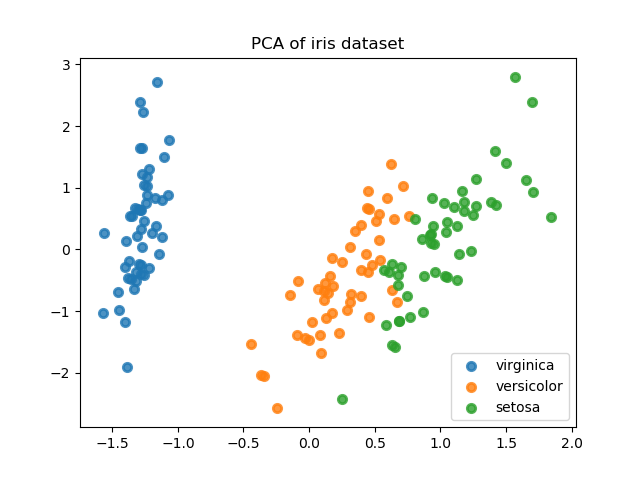
\includegraphics[scale=0.5]{images/iris_PCA.png}
				\caption{PCA Clustering of the Iris Dataset. Visually, we can see that the setosa label has high separability from versicolor and virginica, which are much closer after PCA.}
		\end{figure}
		
		\end{frame}
		
		\begin{frame}
			\frametitle{K Nearest Neighbors Classifier}
			
			\begin{itemize}
				\item Pre-processing:
				\begin{itemize}
					\item We split the data into a 30\% train and 70\% test sets and keep the data balanced.
					\item We also shuffle the data.
					\item We scale the data such that it is within $(0,1)$ using a min-max scaler.
				\end{itemize}
				\item The function class we consider is trivial since it is dependent only on the training data given.
				\item We can view this as a weighting function that weights the $k$-nearest points to the input with $\frac{1}{k}$ and all other points $0$.
				\item Classification Accuracy: 83 percent
				\item Training Accuracy: 91 percent
			\end{itemize}
		\end{frame}
		
		\begin{frame}
			\frametitle{Confusion Matrix for Iris Data}
			
			\begin{figure}
				\centering
				\includegraphics[scale=0.5]{images/confusion_matrix_iris.png}
				\caption{Confusion Matrix of Iris Data. We see that setosa is classified perfectly, while versicolor and virginica have some errors in classification.}
		\end{figure}
		\end{frame}
		
		\begin{frame}
		\frametitle{Persistence Diagrams of Iris Features: Setosa}
		
		\begin{figure}
				\centering
				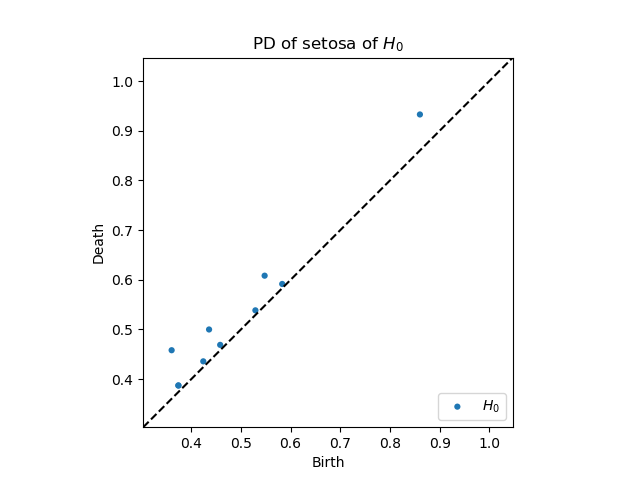
\includegraphics[scale=0.5]{images/PD_H0_setosa.png}
				\caption{Persistence Diagram for Setosa}
		\end{figure}
		\end{frame}

		\begin{frame}
		\frametitle{Persistence Diagrams of Iris Features: Versicolor}
		
		\begin{figure}
				\centering
				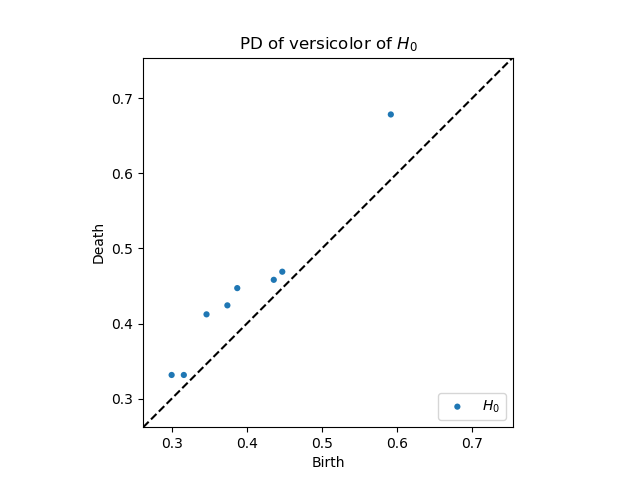
\includegraphics[scale=0.5]{images/PD_H0_versicolor.png}
				\caption{Persistence Diagram for Versicolor.}
		\end{figure}
		\end{frame}
		
		
				\begin{frame}
		\frametitle{Persistence Diagrams of Iris Features: Virginica}
		
		\begin{figure}
				\centering
				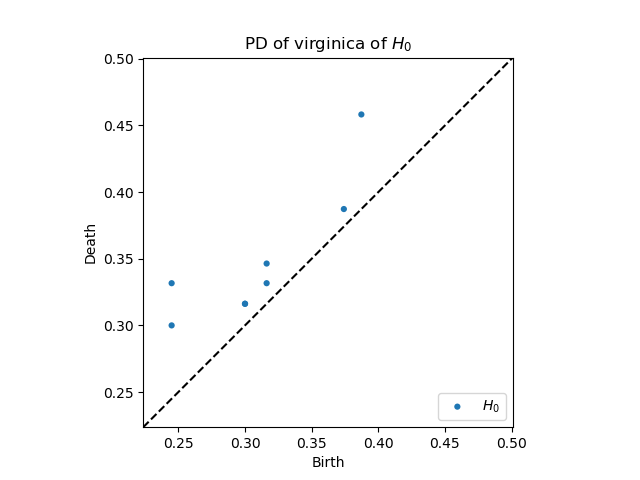
\includegraphics[scale=0.5]{images/PD_H0_virginica.png}
				\caption{Persistence Diagram for Virginica.}
		\end{figure}
		\end{frame}
		
		\begin{frame}
		\frametitle{Pairwise Bottleneck Distances}
		
		\begin{itemize}
			\item The bottleneck distances for each of the iris varieties:
				\begin{itemize}
					\item With themselves: 0 (control)
					\item Setosa, Virginica: 0.04335675
					\item Setosa, Versicolor: 0.04335675
					\item Virginica, Versicolor: 0.04331252
				\end{itemize}
		\end{itemize}
		
		A downside to the Bottleneck Distance as a measure is that quantitatively it can be hard to distinguish for simple data what a good distance is.
		\end{frame}
		